\documentclass[12pt,a4paper]{article}
\usepackage[textheight=28cm,textwidth=19cm,headheight=10mm,footskip=10mm]{geometry}
\usepackage[UTF8]{inputenc}
\usepackage[T1]{fontenc}
\usepackage[french]{babel}
\usepackage{fourier}
\usepackage{amsmath,amsfonts,amssymb}
\usepackage{paralist,array}
\usepackage{pgf,tikz}
\usetikzlibrary{shapes,snakes,arrows}
\usepackage{graphicx,multicol,varwidth}
\usepackage{pstricks-add}

\pagestyle{empty}

\newcommand{\ent}[4]{\begin{flushleft}
\underline{#1}
\hfill
\underline{#2$^{\text{ème}}$ #3}
\vspace{12 pt}
\end{flushleft}
\begin{center}
\begin{LARGE}
\textbf{\underline{\'Evaluation sur Scratch n°#4}}
\vspace{6 pt}
\end{LARGE}
\end{center}}
%fin de la commande \ent (entête du contrôle)

\renewcommand{\arraystretch}{1.5}

\begin{document}
\ent{\textit{date à mettre}}{3}{}{2}
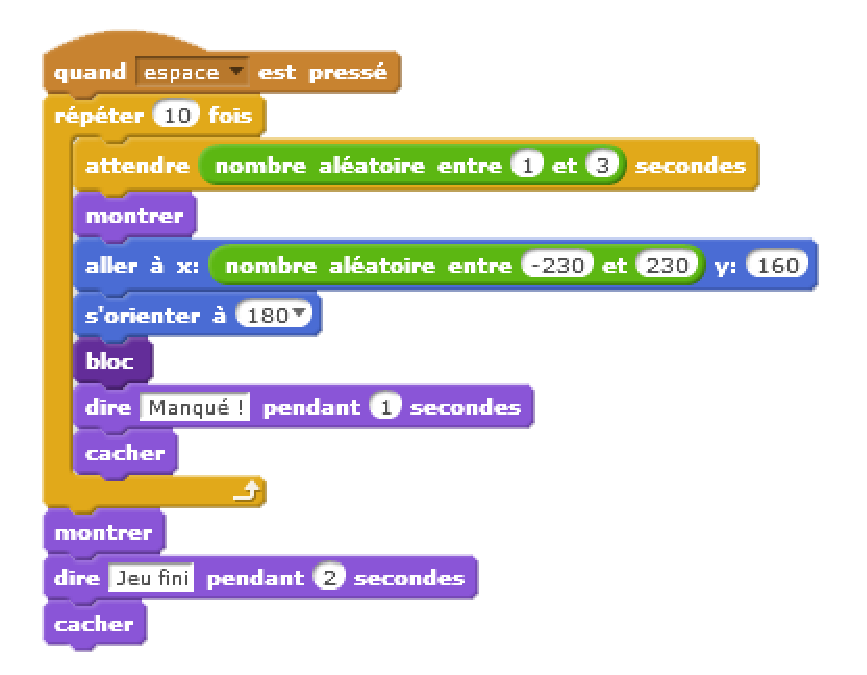
\includegraphics[scale=0.5]{Evaluation2a_Script.eps} \hspace*{3cm}
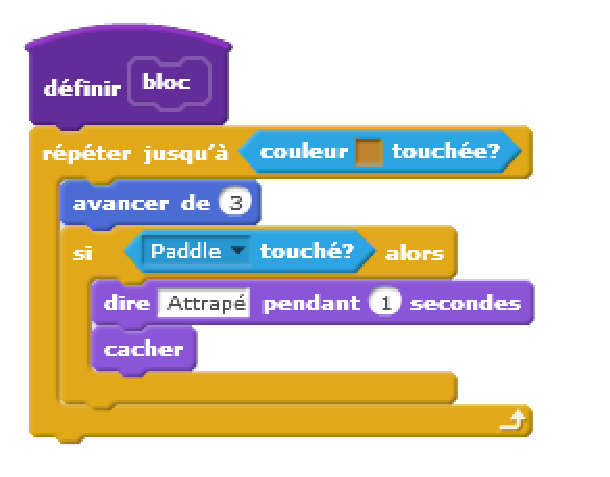
\includegraphics[scale=0.5]{Evaluation2b_Script.eps} \vspace{3pt}
\begin{enumerate}[1{)}]
\item
\begin{enumerate}[a{)}]
\item
Quelle instruction donne la direction de déplacement de la balle ? \vspace{6pt} \\
.\dotfill \vspace{9pt}
\item
Quelle est la vitesse de la balle ? \vspace{6pt} \\
.\dotfill \vspace{9pt}
\item
Combien de balles sont lancées ? \vspace{6pt} \\
.\dotfill \vspace{9pt}
\item
Que signifie l'instruction \og nombre aléatoire entre 1 et 3 \fg{} ? \vspace{6pt} \\
.\dotfill \vspace{9pt}
\item
Décrire l'instruction \og bloc \fg{}. \vspace{6pt} \\
.\dotfill \vspace{6pt} \\
.\dotfill \vspace{6pt} \\
.\dotfill \vspace{6pt} \\
.\dotfill \vspace{6pt} \\
.\dotfill \vspace{6pt} \\
.\dotfill \vspace{9pt}
\end{enumerate}
\item
Un autre lutin \og Paddle \fg{} se déplace uniquement horizontalement. \vspace{3pt} \\
Si on appui sur la flèche de gauche, il se déplace vers la gauche de 10 pas. \vspace{3pt} \\
Proposer un script permettant à ce lutin de se déplacer vers la gauche. \vspace{6pt} \\
.\dotfill \vspace{6pt} \\
.\dotfill \vspace{6pt} \\
.\dotfill \vspace{6pt} \\
.\dotfill \vspace{6pt} \\
.\dotfill \vspace{6pt} \\
.\dotfill 
\end{enumerate}
\vfill
NOM - Prénom : \dotfill 


\end{document}